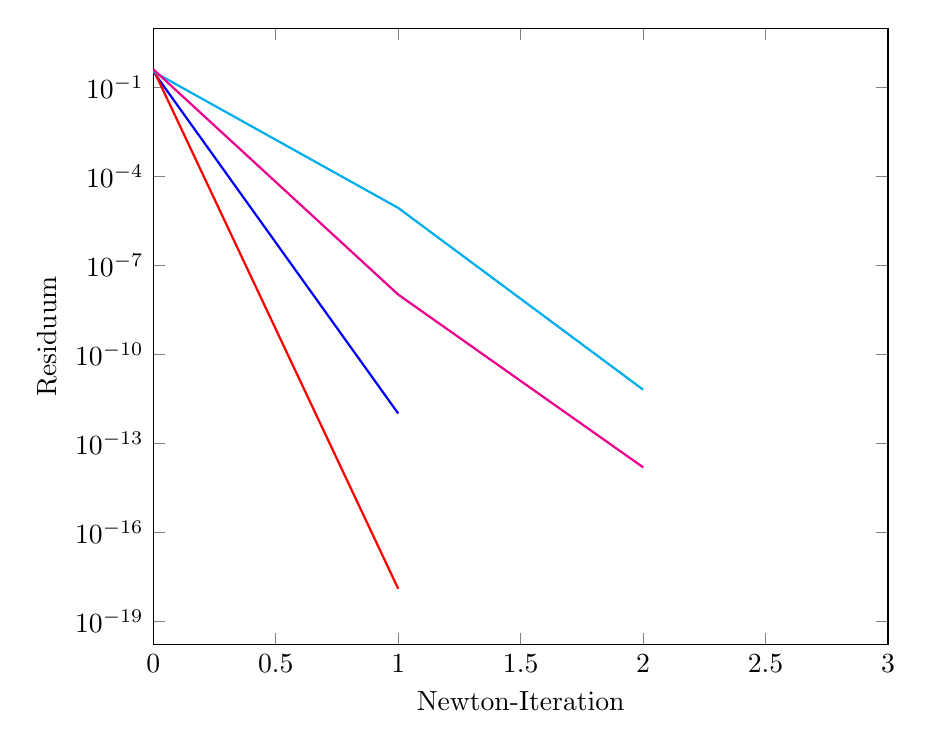
\begin{tikzpicture}[every plot/.append style={thick}] 
\begin{axis}[ 
label style={font=\normalsize}, 
xlabel={Newton-Iteration}, 
ylabel={Residuum}, 
xmin=0, xmax=3, 
ymode=log, 
ymin=0, ymax=10, 
width=0.9\textwidth, 
grid style=dashed, 
] 
\addplot[ 
color=blue, 
] 
coordinates { 
(0, 3.44e-01)(1, 1.00e-12)}; 
\addplot[ 
color=red, 
] 
coordinates { 
(0, 4.07e-01)(1, 1.22e-18)}; 
\addplot[ 
color=cyan, 
] 
coordinates { 
(0, 3.44e-01)(1, 8.64e-06)(2, 6.38e-12)}; 
\addplot[ 
color=magenta, 
] 
coordinates { 
(0, 4.09e-01)(1, 1.03e-08)(2, 1.53e-14)}; 
\end{axis} 
\end{tikzpicture} 
